\documentclass{article}
\usepackage{amsmath}
\usepackage{graphicx}
\title{Investing notes}
\date{10-19-2022}
\author{Tommy Bui}

\begin{document}
	\maketitle
	\newpage
	\pagenumbering{arabic}

	\section{Analyzing a stock from Yahoo Finance} 
	
	\begin{figure}[h!]
		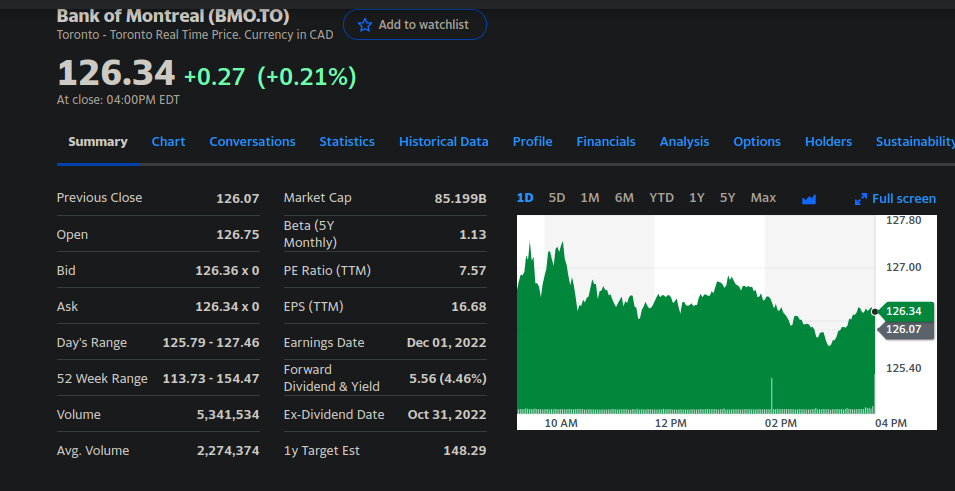
\includegraphics[width=\linewidth]{InvestingPics/figure1.png}
		\caption{View of \$BMO.TO in Yahoo Finance}
		\label{fig:chart1}
	\end{figure}

	%Figure \ref{fig:chart1} is a chart of BMO.TO

	\subsection{Analyzing the Summary Tab}

	\begin{itemize}
		\item {\bf Previous Close:} represents the last closing price reported of a security during a given time period; A security's previous close is an important value that is used by investors to chart gap patterns which can show substantial changes from a previous close to a new open.
		\item {\bf Open:} AKA the opening price; this is the value that a security is initially valued when the exchange opens for the day.
		\item {\bf Bid:} AKA the bidding price; A bid is an offer made by an investor, trader, or dealer in an effort to buy an asset or compete for a contract; The spread between the bid and asking price is a reliable indicator of supply \& demand for the security.
		\item {\bf Ask:} AKA asking price; The price at which someone is willing to sell a security for.
		\item {\bf Range:} Refers to the difference between the highest \& lowest prices a security or index ranges over an interval of time.
		\item {\bf Volume:} Trading volume is a measure of how much a given asset has been traded over a period of time. For stocks, volume is measured in the number of shares traded, for futures \& options, volume is based on how many contracts have changed hands. Volume can indicate market strength, as rising markets on increasing volume are typically viewed as strong and healthy.
		\item {\bf Avg. Volume:}
		\item {\bf Market Cap:} Market capitalization is calculated by multiplying the number of shares outstanding by the current price of a single share (i.e. A company with 50 mil shares \& a stock price \$100 per share would have a market cap of \$5 bil). Market cap is a metric based on stock price. \underline{Market capitalization is used to help define the value of a company when analyzing potential trade opportunities}. 
		\item {\bf Beta (5Y monthly):} Beta measures how volatile a stock is in relation to the broader stock market over the last 5 years, using one data point per month. A stock with a high beta indicates it's more volatile than the overall market and can react with dramatic share-price changes amid market swings. 
			\begin{itemize}
				\item A beta of one means that an investment is as volative as the rest of the market. If the security has a beta of two, it means that the stock is twice as volatile as the market. 
				\item Low risk traders often avoid investing in high-beta stocks.
				\item Beta relies on past information and so doesn't help describe the fundamentals of the security, however a beta may be a strong factor in quantifying risk for frequent traders
			\end{itemize}
		\item {\bf Price-to-Earnings (P/E) Ratio:} The price-to-earnings (P/E) ratio relates a company's share price to its earnings per share.
			\begin{itemize}
				\item The ratio represents the factor which traders are willing to buy the security compard to the profit gained by the company with the sale of the security.
				\item A high (P/E) ratio could mean that a company's stock is overvalued OR that investors are expecting high growth rates in the future.
				\item According to investopedia, a P/E ratio holds the most value to an analyst when compared against similar companies in the same industry or for a single company across a period of time.
				\item {\bf NOTE:} Valuation ratios compare the company's market value with some financial aspect of its performance - earnings, sales, book value, cash flow, and so forth; the ratio-based approach is the most commonly used method for valuing stocks since ratios are easy to calculate and readily available. The downside of making sense of valuatio ratios is that they require a quite a bit of context (i.e. A P/E ratio of 15 does not mean much unless you know the P/E of the market as a whole, the P/E's of the company's main competitors, the company's historical P/E's, and similar information.
				\item These two types of EPS metrics factor into the most common P/E ratios: the {\bf forward P/E} and the {\bf trailing P/E}.
				\item The forward (or leading) P/E uses future earnings guidance rather than trailing figures. Sometimes called "Estimated price to earnings", this
					forward indicated is useful for comparing current earnings to future earnings and helps provided a clear picture of what earnings will look like.
				\item The main issue with forward P/E metric is that companies could underestimate earnings in order to beat the estimate P/E or may overstate the estimate and later adjust it going into their next earnings annooucement.
				\item Trailing Price-to-Earnings relies on past performance by dividng the current share price bye the total EPS earnings over the past 12 months; it's the most popular P/E metric because its the most objective (assuming companies reported their earnings accurately)
				\item The trailing P/E has its share of shortcomings as well, namely, that a company's past performance doesn't reflect future behavior; thus investors should commit money based on future earnings power, not the past.
				\item If an EPS remains constant, while the stock pricecs fluctuate, is a problem. If a major company event drives the stock prices higher or lower, the trailing P/E will be less reflecitve of thos changes.
				\item If the forward P/E is lower than the trailing P/E, it means analyst expect earnings to increase; if the foward P/E is higher than the current P/E, analysts expect them to decrease
				\begin{align*}
					Price-to-Earnings (P/E) ratio &= \frac{Market Value Per Share}{Earnings Per Share}\\
				\end{align*}
				\item Consider this example where we compare two financial company's P/E ratio to determine which is over/undervalued:
					\begin{itemize}
						\item Bank of America Corporation \$BAC closed out the 2020 year with the following:
							\begin{itemize}
								\item {\bf Stock Price} = \$30.31
								\item {\bf Diluted EPS} = \$1.87
								\item ${\bf P/E} = 16.21 = (\$30.31/\$1.87)$
							\end{itemize}
						\item In short, \$BAC was traded at roughly 16 times its trailing earnings
					\end{itemize}
			\end{itemize}
	\end{itemize}

\end{document}
